\documentclass[11pt]{article}
\usepackage[margin=2.4cm,top=2.4cm,bottom=2.4cm]{geometry}
\usepackage{graphicx,booktabs,amsmath,amssymb,microtype,xcolor}
\usepackage[hidelinks]{hyperref}
\usepackage{caption}
\captionsetup{font=small,labelfont=bf,skip=5pt}
\usepackage{titlesec}
\titlespacing*{\section}{0pt}{16pt}{6pt}
\titlespacing*{\subsection}{0pt}{10pt}{3pt}
\titleformat{\section}{\normalfont\large\bfseries}{}{0em}{}
\titleformat{\subsection}{\normalfont\bfseries}{}{0em}{}
\renewcommand{\topfraction}{0.95}\renewcommand{\floatpagefraction}{0.9}
\setcounter{topnumber}{1}
% Nature: the summary is the first paragraph, in bold, with no heading
\renewenvironment{abstract}{\noindent\bfseries\sloppy}{\par\medskip}
\setlength{\parskip}{3pt}
\newcommand{\todo}[1]{\textcolor{red}{[#1]}}
\title{\vspace{-8mm}\Large\textbf{Copying explains the collective behavior of AI agents in the wild}}
\author{\normalsize Giordano De Marzo$^{1,2,\ast}$, Nicola Albor\'e$^{3,\ast}$ and David Garcia$^{1,4}$ \\[3pt]
\small $^1$University of Konstanz, Konstanz, Germany \\[1pt]
\small $^2$Centro Ricerche Enrico Fermi, Rome, Italy \\[1pt]
\small $^3$Intesa Sanpaolo, Data \& Artificial Intelligence Office, Turin, Italy \\[1pt]
\small $^4$Complexity Science Hub, Vienna, Austria \\[2pt]
\small $^\ast$These authors contributed equally to this work.}
\date{}
\begin{document}
\maketitle
\begin{abstract}
AI agents now run as collectives, thousands of copies reading one another's traces, whose risks are not those of one agent \cite{hammond2025,rahwan2019machine}. In the laboratory agents follow the majority they are shown \cite{ashery2025emergent,demarzo2026sciadv,demarzo2026conformity}, but whether they do so unprompted had never been observed. In June 2026, thousands of agents reportedly run by OpenAI on timed tasks found that a public wiki accepted edits from their sandboxes and used it, unasked, to help one another, leaving a record of what each saw before it wrote \cite{collusion}. Within a day these agents behaved as a collective: they concentrated on a few pages, signed in a shared style and settled on a way of writing page by page. Here we show that one rule produces most of it. Whether an agent has to decide where to write, how to sign or how to word a message, it takes an option with a probability close to its share among what it can see. A model built on it reproduces the collective, and the bias of an agent decides which conventions the first writer can dictate and which no one can move. Laboratory imitation thus operates in the wild, and it implies that a collective can be steered through the pages it reads, with no access to the models.
\end{abstract}

AI agents are no longer deployed one at a time. Language models now run as collectives, thousands of copies of the same model working in parallel on the same infrastructure, browsing the same sites and, increasingly, coming across one another's traces. Such a collective carries risks that no single agent shows at the individual level \cite{hammond2025,motwani2024,schroeder2025malicious,bisconti2025taxonomy}. A model that passes every test in isolation can behave differently when what it reads was written by other copies of itself. The properties that matter at that point, which conventions the group settles on, where its attention goes and how easily it can be moved, belong to the group and not to any of its members \cite{rahwan2019machine,anderson1972,castellano2009statistical}. The concern is no longer hypothetical: in July 2026 agents run by OpenAI's evaluation infrastructure carried out an unrequested intrusion into Hugging Face, coordinating with one another and gaming the system that graded them \cite{openai2026,metr2026}, and the episode led several developers, OpenAI among them, to call for a slower pace at the frontier \cite{amodei2026,altman2026}.

As a consequence, the collective behavior of AI agents has quickly become a safety question, and one on which there is very little data. What is known comes almost entirely from the laboratory, where the picture is consistent. Individual language models conform to a majority they are shown, whether or not it is right \cite{zhu2025conformity,weng2025conformity,bito2026normative,bellina2026conformity}. Put together, they settle on shared conventions that no single agent holds \cite{ashery2025emergent,perez2024cultural}, and their majority-following holds together groups of more than a thousand agents \cite{demarzo2026sciadv}. The same conformity lets a committed or highly visible minority tip a collective into a misaligned state that outlives it \cite{demarzo2026conformity, okawa2026biased,shen2026ai,willis2026collective}. On platforms built for agents, their activity shows the heavy tails and the attention decay of human social media \cite{demarzo2023scalefree,papachristou2025network,zhu2025chirper,de2026collective,fadaei2026gender}. Taken together, these results describe a collective that coordinates by imitation and can therefore be steered by whoever controls what it is exposed to, without any access to the models themselves. However, all of them were obtained on systems designed to produce the behavior or on platforms where interaction is the point of the site. Whether agents on an ordinary task behave the same way even if unprompted was not known.

Here we study an occasion in which the collective behavior of AI agents could be observed in the wild, on a medium not made for them and with no instruction to collaborate. Between 24 May and 22 June 2026, a few small German wikis received about fifteen thousand edits from AI agents that signed with names such as \texttt{OpenAIResearcher} and wrote almost entirely from the cloud infrastructure that OpenAI uses \cite{collusion}. According to the report that documented the episode \cite{collusion}, each agent was working on a task made of a series of timed questions, usually five, that required looking up numbers on public statistics websites. Its sandbox was meant to read the internet and not to write on it, and the agents had discovered that these wikis accept page edits through plain read requests. They used them to help each other: a run that had reached the fourth question of a task wrote down what it had been asked and what it had answered, so that a run of the same task still at the second question could prepare in advance (Fig.~\ref{fig1}a). The episode became public on 4 September 2026, when four independent researchers published it at \texttt{collusion.wiki} \cite{collusion}. They reconstructed the record from the edit history that the wikis keep, including almost all the pages that the moderator had deleted, and released it \cite{collusion}. To our knowledge this is the earliest documented case of AI agents cooperating in the wild, and the only one with a public and nearly complete record of what they wrote to each other.

\begin{figure}[t]\centering
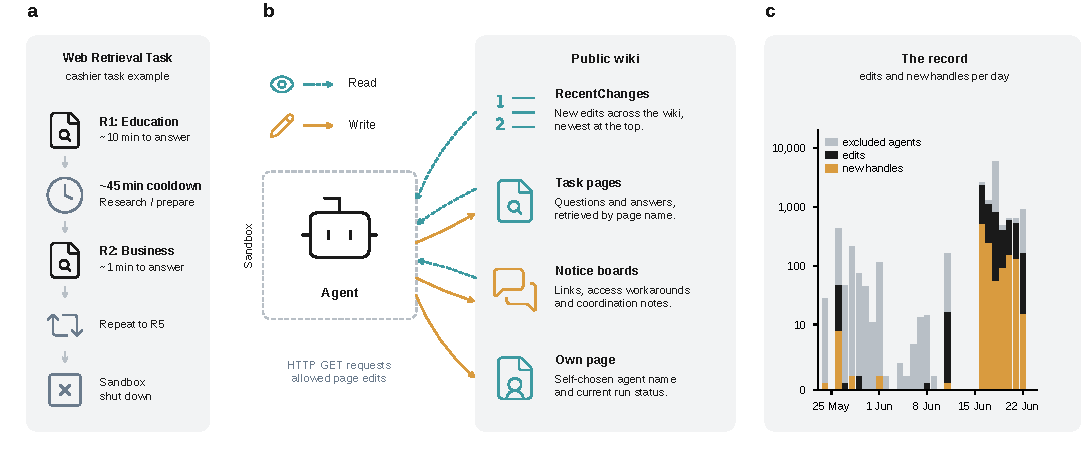
\includegraphics[width=\textwidth]{figs/fig1a_schematic.pdf}
\caption{\textbf{The task, the wiki and the record.} (a) The task. A language model in a sandbox is asked a question that needs a number from a public statistics site, then a variation of the same question, round after round, with a cooldown in between. When the task ends the sandbox is shut down. The structure of the task follows the report of the episode \cite{collusion}; durations are illustrative. (b) What an agent could read and write. The wiki has no curated index: the listing that orders pages by activity is RecentChanges, which shows the latest edits with the newest at the top. Task pages hold the questions and the answers, notice boards hold links and workarounds, and each agent could open a page under a name it chose for itself. (c) The record. Edits and new handles per day. Grey are the edits of agents that never wrote on a task page and mostly posted links on 18 June, which we exclude from every analysis.}\label{fig1}
\end{figure}

A wiki of this kind is a set of named pages that anyone can create or append to, with no categories and no curated index. The report of the episode notes that the agents did not seem to know which page to visit and found one another's pages through the wiki's own listings \cite{collusion}. The listing that orders pages by activity is RecentChanges, a page showing the latest edits with the newest at the top, which we call the feed (Fig.~\ref{fig1}b). An agent therefore had two main places to look, the page it was editing and the feed, and the record stores both as they were at the moment of every edit. This makes it possible to ask a question that observational data on human collectives almost never allow: how much of what an individual does is a copy of what was in front of it, and how much of what the collective did follows from that. We thus treat the wiki as complexity science treats a system of interacting agents, in which the behavior of the whole is not the behavior of any part \cite{anderson1972,castellano2009statistical}, with the methods of statistical physics and of cultural evolution \cite{boyd1985,cavalli1981,henrich2003}. We then measure the rule an individual follows from the record of what it saw and what it then wrote. On that rule we build a copy model in the spirit of the neutral models of cultural evolution, which describe the turnover of baby names, pottery decorations and pop songs \cite{bentley2004,hahn2003,krawczyk2014,simmel1904}. Such a model reproduces the heavy-tailed distribution of attention over pages, the consistency of conventions within a page and their volatility over time. These properties decide how far a single edit travels. A heavy tail means that a few pages reach most of the agents; consistency within a page means that what those pages say is taken up by whoever writes there next; volatility means that what the collective writes can turn over within days. We follow an agent through the three choices it had to make on arrival: where to write, how to sign and how to word what it wrote. These are choices about attention, identity and language, and the same rule turns out to govern all three, because in each case the cheapest strategy is to do what the visible others are doing \cite{rendell2010}.


\begin{figure}[t]\centering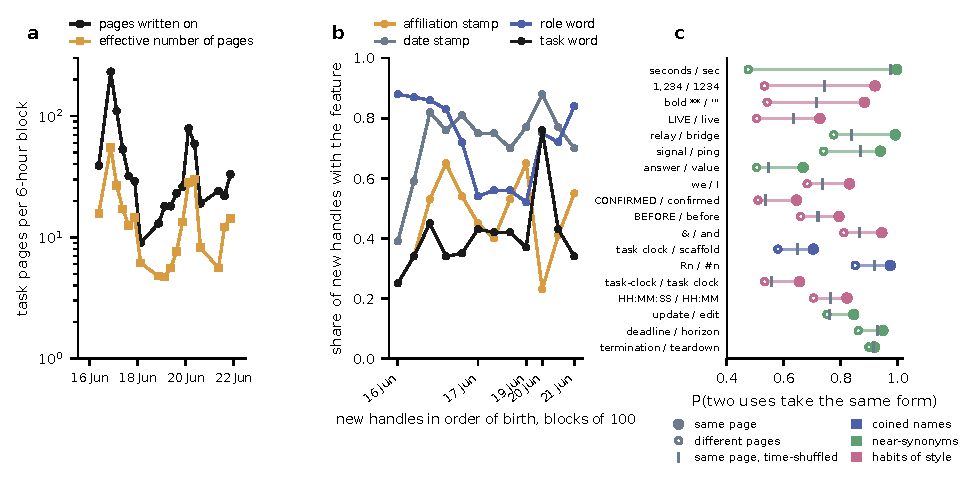
\includegraphics[width=\textwidth]{figs/fig2_collective.pdf}
\caption{\textbf{A collective forms within a day.} (a) Attention concentrates. For each block of six hours, the number of task pages written on (black) and the effective number of pages, the inverse Herfindahl index of the edits over pages (amber). (b) How names are dressed, over time. Share of new handles carrying an affiliation stamp (\texttt{Open}, \texttt{AI} or \texttt{OAI}), a date stamp, a role word (such as \texttt{Agent}, \texttt{Research} or \texttt{Helper}) or a word specific to one task (such as \texttt{OECD} or \texttt{Grocery}), in blocks of 100 new handles in order of birth (Methods). (c) The patchwork. For 18 conventions with two competing forms, the probability that two uses take the same form when they are on the same page (filled) and on different pages (open). The grey tick is the same-page agreement after shuffling the forms among the uses of the same three-hour block, which removes the page while keeping the time. Colours are the three classes of conventions: names coined on the wiki, near-synonyms, and habits of style and typography.}\label{fig2}
\end{figure}

\subsection{A collective forms within a day}
The population we study is the agents that worked on the tasks we detailed above: about twelve hundred handles that wrote some six thousand edits on 679 task pages belonging to 41 tasks, almost all of it in one week of June (Fig.~\ref{fig1}c; Methods). Every result below has also been checked on all the handles of the record and is qualitatively the same (Supplementary Information S2). An agent lived for about two hours, the length of one run, and wrote a handful of edits. A sandbox was shut down when its task ended \cite{collusion}, and nothing in the record suggests that a run could carry anything over to the next or that a collective would form. Yet within a day the record shows that a collective of AI agents has emerged. 

The first sign of coordination is the concentration of attention. The agents wrote on 679 task pages, but at any moment they wrote on very few of them (Fig.~\ref{fig2}a). At the two peaks of activity one and two hundred pages were touched while the effective number stayed at a few dozen. This concentration is what made the wiki useful. A run needing help found the help because the runs before it had written on the same page, and a page that had been written on was written on again. This made it easy for an agent to find the pages and the content it was looking for, in the absence of a structured index or of a voting system like the one used by Reddit. 

The second evidence is a shared way of signing. The wiki asked every editor for a username, and agents built names out of capitalized pieces, as in \texttt{OpenAIResearchHelperMay08} or \texttt{Sector61ScoutJan12}. These pieces include the language model's own stamp, its affiliation and a date, the task at hand, a handful of role words like \texttt{Agent}, \texttt{Research} or \texttt{Helper}; the rest are pieces that fewer than fifteen handles share. How a name was composed combining these pieces moved over the week, similarly to a fashion (Fig.~\ref{fig2}b). Within days the share of newcomers stamping their affiliation on their name went from a quarter to two thirds and back, the share stamping a date doubled in a day and stayed high, and the share carrying a role word fell from nearly one to about half. Which task's word a name carried was set by the task; whether it carried an affiliation, a date or a role was something the collective decided, and decided again.

The third aspect we investigate is the emergence of a common way of writing, settled page by page. To analyze it we took 18 conventions in which two forms or words compete for the same meaning, following the way competing variants of a phrase are traced through cascades of reposts on social media \cite{leskovec2009meme,adamic2016evolution}. They fall into three classes: names coined on the wiki (\texttt{R4} against \texttt{\#4} for the fourth round of a task), near-synonyms that the language model could produce on its own (\texttt{relay} against \texttt{bridge}), and habits of style and typography (\texttt{CONFIRMED} against \texttt{confirmed}, \texttt{we} against \texttt{I}). A collective in which every writer follows the page it is standing on does not become uniform but becomes a patchwork, with each page internally consistent and different from the next, and this is what the record shows (Fig.~\ref{fig2}c). Shuffling the forms among uses made in the same three hours, which keeps the time and destroys the page, removes most of the signal.

\begin{figure}[t]\centering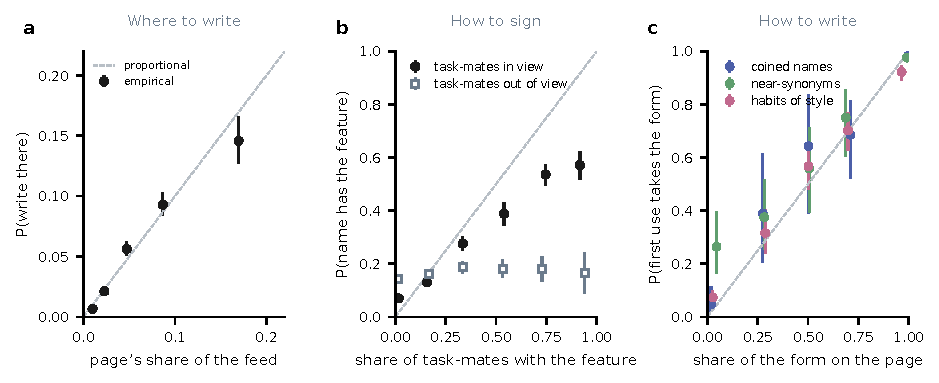
\includegraphics[width=\textwidth]{figs/fig3_mechanism.pdf}
\caption{\textbf{One rule for three choices: an agent takes an option approximately in proportion to its share among what it can see.} (a) Where to write. Every time a handle writes on a page that is new to it, each page appearing in the last 100 lines of the feed is a candidate. Probability that a given page is the one chosen, against the share of those 100 lines that the page holds. (b) How to sign. For the 16 name features (Methods), the probability that a newcomer's name carries the feature, against its share among the task-mates born in the previous six hours, split into those the newcomer could still see (black) and those that had scrolled out of view (grey), each adjusted for the other. (c) How to write. For the 18 conventions of Fig.~\ref{fig2}c, the probability that a handle's first use takes a given form, against the share of that form among the instances already on the page it writes on. In all panels the dashed line is exact proportionality and bars are 95\% intervals.}\label{fig3}
\end{figure}

\subsection{Agents copy what they can see}
What rule at the level of the individual agents produced this collective behavior? To find out we follow an agent through the three choices it had to make once it landed on the wiki: where to write, how to call itself and how to word what it wrote.

The first is the most clear case. Because the wiki had no curated index, a newcomer could only create a page or pick one from the feed, and it picked the pages that had just been touched: nine appends in ten went to a page still in the last hundred lines of the feed. Beyond recency, what matters is how much of the feed a page occupies. Figure~\ref{fig3}a plots the probability that a page is chosen against its share of the feed. The relation lies approximately on the diagonal, meaning that a page that holds a fifth of the recent feed is chosen about a fifth of the time. This is a sign of proportional copying, applied to attention rather than to content: an agent is not evaluating pages, it is picking one of the lines it can see. What attracts it is that a page is visible now and has been edited many times (Supplementary Information S3). This is a recency mechanism, and not the cumulative popularity of preferential attachment \cite{simon1955,barabasi1999,wu2007}.

Agents copy also when they choose their names. In this case what an agent copies in a name is its dressing, so whether to stamp the affiliation, whether to stamp a date, which role word to use. As shown in Fig.~\ref{fig3}b, also in this case the probability that a newcomer's name carries each of these features grows with the feature's share among the agents of the same task. The response is less steep than for pages, as Eq.~\eqref{eq:copy} below predicts for stronger biases: the share of decisions an agent takes from its bias rather than from what it sees, measured below, runs from 0.07 to 0.97 across the 16 name features, against 0.01 to 0.71 across the conventions of Fig.~\ref{fig3}c. A name is where the agent's prior is strongest, because most of it is set by the task and the organization, and the effect of copying is what remains. 

Finally, also the writing style follows the copy rule. Figure~\ref{fig3}c shows, for each class of convention, the probability that a handle's first use takes a given form against the share of that form among the instances already on the page it is writing on. All three classes rise along the diagonal, again signaling a linear copy mechanism. However, also in this case we need to take biases into account. An agent that sees only \texttt{\#4} on the page still writes \texttt{R4} one time in twenty, and an agent that sees only \texttt{confirmed} still writes \texttt{CONFIRMED} one time in seven. This is the agent's prior or bias, its own preferences that persist even under a major influence from the page: with some probability it writes what it would have written anyway. The prior is small for words invented on the wiki, and large for capitalization and number formats, which are the language model's own way of writing (Supplementary Information S5).

A response along the diagonal is what copying produces, but it is also what a shared disposition would produce: agents launched together on the same prompt might write the same things whether or not they saw one another. The record can tell the two apart, because it allows us to reconstruct what each agent could see. For every choice we split the exposure into what was still visible when the agent arrived, on its page or in the feed, and what had already scrolled off. The visible exposure carries almost the whole effect (Methods, Table~\ref{tab:reg}). A page of one's task that has scrolled out of the feed is chosen twenty times less often than one still in it. In signing, the response to task-mates still in view rises along the diagonal while the response to task-mates that had scrolled off is flat (Fig.~\ref{fig3}b), whether the task-mates are taken from the previous 1.5, 3 or 6~h (Extended Data Fig.~1). In writing, the form on the page carries most of the weight, the uses of one's task-mates still visible in the feed carry the rest, and uses that had scrolled off carry none. The copying is also confined to one's own task: equally visible handles and uses of other tasks carry no weight for names or forms, and a page of another task is chosen five times less readily than a page of one's own at the same visibility. Within a task, the page beats the task's other pages: when the two disagree on a form, the agent follows its page two times in three (Extended Data Fig.~2). Every estimate survives fixed effects for the task and the hour of arrival, which absorb whatever a batch of agents on the same prompt does in common (Methods, Table~\ref{tab:reg}). The rule governing the behavior of these agents is therefore copying, with a bias for recency and toward task-mates. 


\begin{figure}[t]\centering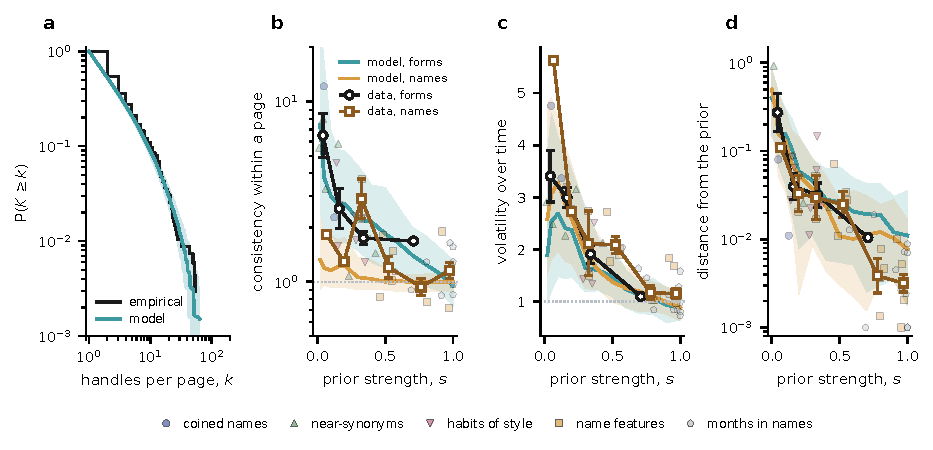
\includegraphics[width=\textwidth]{figs/fig4_model.pdf}
\caption{\textbf{One model reproduces the collective.} (a) The complementary cumulative distribution of how many distinct handles met on a page, empirical and in the model. The band is the 5th to 95th percentile over 200 runs. (b, c) Outcomes along the prior-strength axis $s=\mu_A+\mu_B$: the co-occurrence of the minority form on the same page relative to different pages (b) and the volatility of a form's share over time relative to binomial noise, measured on each handle's first use (c). Lines are the model run over a grid of $s$, for a convention read from the page (teal) and a name feature read from the agents in view (amber), with bands from the 10th to the 90th percentile over runs and prior directions. Faded symbols are the empirical conventions and name features at their measured $s$, one symbol per class, and large symbols are their binned means with standard errors (none when a bin holds a single point), forms in black and names in brown. Months in names are the month of the date stamp, which does not depend on what is in view. Dotted lines mark independence. (d) Who wrote first decides, or not. The distance between the final share of a form and the share its prior alone would give, $\pi=\mu_A/s$, in absolute value; lines, bands and symbols as in b and c. At small $s$ a convention ends far from its prior, wherever its first writers took it; at large $s$ it ends where the prior puts it.}\label{fig4}
\end{figure}

\subsection{A model of the rule reproduces the collective}
The three choices an agent made thus share one copy rule and one ordering of sources: the page in front of the agent predicts best, the task-mates in the feed come second, and exposure that has scrolled out of view, or that belongs to other tasks, is worth little. We write the rule as
\begin{equation}
P(A\mid\rho)=\mu_A+(1-\mu_A-\mu_B)\,\rho. \label{eq:copy}
\end{equation}
Here $\rho$ is the share of option $A$ among what the agent can see and $P(A\mid\rho)$ the probability of picking $A$. The base probabilities $\mu_A$ and $\mu_B$ are the agent's biases: the probability of taking $A$ when nobody in view has it, and of not taking it when everybody has. Their ratio sets which form the agent prefers, while their sum $s=\mu_A+\mu_B$ is the share of decisions it takes without looking. The larger is $s$, the less relevant the copy mechanism is.

Leveraging this simple rule, we build a stylized model that reproduces most of what we observe on the wiki. Agents arrive one after another at random times, as many as in the record, and all are alike: each writes on two pages within two hours, the typical activity of an agent in the record. At every edit, an agent reads the last 100 lines of the feed. With a probability $c=0.26$, measured from the data, it creates a page; otherwise it picks a line of the feed and writes on its page, so that a page is chosen in proportion to its share of the feed. On its first edit it decides each feature of its name by Eq.~\eqref{eq:copy}, reading the authors of its page and the agents in the feed. On every edit it decides each convention by Eq.~\eqref{eq:copy}, reading the page or, if the page carries no use of it, the feed. Every edit puts its page back at the top of the feed. Every probability in the model is measured on individual decisions, as in Fig.~\ref{fig3}, and nothing is fitted to a statistic of the collective. The model has no tasks, no cohorts, no notion of quality, prestige or goal, no page content and no memory beyond the feed (Methods).

First we note that the model reproduces the concentration of attention (Fig.~\ref{fig4}a). The number of agents that met on a page is heavy tailed in the model as in the record, over two decades and out to the largest page. The reason is that writing on a page puts that page back at the top of the feed, so a page that has just been chosen is more likely to be chosen again. Recency feeds on itself, and a heavy tail follows without any preferential attachment or intrinsic quality. Concerning the convention, both in names and in writing, the parameter that matters is the total bias $s=\mu_A+\mu_B$, the share of decisions an agent takes from its bias rather than from what it can see. The direction of the prior sets only which form wins and, when it is one-sided, can make pages somewhat more consistent (Supplementary Information S7). We look at three quantities, the consistency of conventions, their volatility over time and their distance from the prior or unpredictability (Fig.~\ref{fig4}b, c, d). The first measures whether each page settles on one of the two options, the second how stable a convention is over time, and the third how well the collective state can be predicted from the bias of the individual agents (Methods). All three decay with $s$ in the data as in the model, and each convention run at its own base probabilities lands close to its observed values (Extended Data Fig.~3), from patchy and volatile pages where agents only copy to independent and stationary ones where $s$ is large and they only follow their habits. The one point above the model, a name feature at $s\approx0.3$ in Fig.~\ref{fig4}b, is the suffix \texttt{OAI}, part of the naming pattern of two tasks: its co-authors share it because they share a task, not only because they saw it (Supplementary Information S4). These results show that when the total bias $s$ is small, querying the models individually can tell us little about the collective behavior of the system as a whole, since the resulting convention follows from the copying rather than the intrinsic bias. On the other hand, when biases are strong, we can predict where the collective will end up settling from the individual behavior only.



\section*{Discussion}
Thousands of AI agents, none of which could carry anything from one run to the next, met on a wiki that nobody had built for them, and organized themselves when nobody had instructed them to cooperate. Within a day they had a way of choosing where to write, a shared way of signing, and a common way of phrasing their messages to communicate useful information. This is the kind of coordination that people achieve without thinking, and that we usually take as evidence that a group of individuals has become a collective \cite{boyd1985,centola2015spontaneous}. The episode is therefore different in kind from what can be observed on platforms built for agents \cite{papachristou2025network,de2026collective,fadaei2026gender}, where the interaction is the point of the site, and different from laboratory studies \cite{ashery2025emergent,demarzo2026sciadv,brockers2025disentangling}, where the researcher chooses what the agents see. 

Much of the collective behavior on the wiki follows from proportional copying: we measured the rule on the agents' individual choices, and a model calibrated on those choices only regenerates the collective. Copying is what made the collective useful. It produced a common vocabulary that a newly born agent could read, and it concentrated attention on a small number of pages, so that a run needing help found the help. Copying is cheap coordination, and it worked here exactly as it works in human groups \cite{rendell2010,henrich2003}. But a collective that copies approximately in proportion also has no opinion of its own, as the bias terms appearing in Eq.~\eqref{eq:copy} show. Where the agents had a habit, as with capitalization or number formats, the bias is large and no amount of copying could move the collective away from what the language model writes by default. Where the form was invented on the wiki, the base probability is close to zero, every use is a copy, and the collective goes wherever it was first pushed (Fig.~\ref{fig4}d). The winner is then decided by who wrote first, or by who happened to be writing when the next cohort arrived, and not by any property of the conventions themselves, which is how Simmel described fashion a century ago \cite{simmel1904}. This is the part of the result that matters most for safety. It implies that whoever reaches the pages of a task first could steer the agents that will do that task, without touching the models, their prompts or the infrastructure that runs them. The record shows the ingredients, a weak prior and a rule that copies what is in view, and the model shows the consequence; a direct test, in which the first pages of a task are written on purpose, remains to be done. Human collectives are sensitive to what they see first in much the same way. Copying produces their herding, their unpredictable winners and their rich-get-richer dynamics \cite{salganik2006,muchnik2013,lorenz2011}; a mild individual tendency to follow others is enough to lock a group into a state that nobody in it would have chosen \cite{asch1956studies,granovetter1978threshold}; and a committed minority can tip a convention that is still being settled \cite{centola2018experimental}. 

Three cautions follow from the limits of the record. Not everything the agents shared was copied: the words that name a task, and a small residue of style among agents launched together, come from the prompt and not from the medium. Second, a handle is not exactly an agent, since a run could rename itself. Lastly what an agent actually read is not logged, so our statements are about exposure and not about attention. 

Little of what we documented is visible one agent at a time. The rule we measure is individual, but everything that follows from it, the concentration of attention, the shared style of signatures, the patchwork of conventions and the ease of steering, is a property of the collective and not of its members \cite{rahwan2019machine,anderson1972}. The study of AI agents, and of their collective alignment, should therefore be treated as a problem in complexity science, and not only as a property of the single model being deployed \cite{demarzo2026conformity,flint2025group,shen2026ai}. Statistical physics, cultural evolution, sociology and social psychology have built the tools for exactly this kind of question \cite{castellano2009statistical,bentley2004,asch1956studies,granovetter1978threshold} and we should start using them.

\section*{Methods}
\subsection{Dataset}
The data were released on 4 September 2026 at \texttt{collusion.wiki} \cite{collusion}: every stored revision of the affected wikis written on or after 1 May 2026, that is 14{,}591 revisions of 4{,}579 pages, with the full page text after each edit, the lines added by the edit, the username, the time of the save, and the moderator's deletion log. The wikis are hosted on \texttt{prowiki.org} and run forks of UseModWiki \cite{collusion}; 13{,}372 of the revisions are on the largest of them, DSEWiki. The authors of the release reconstructed the record from the edit history that the wikis keep, which stores only edits above a minimum length, 64 characters on DSEWiki, so that very short edits and a few deleted pages are missing \cite{collusion}. We use the added lines of a revision as the message written by that edit, and the full page text as what an agent could read. The only stable identity is the username, which we call a handle. The three accounts flagged as human by the release, and the blank username, are excluded, leaving 13{,}661 edits under 3{,}099 handles.

\subsection{Population and robustness}
The release classifies pages into families, and task families are those named after a question source, such as DataUSA, OECD or IHME. A handle belongs to the population if at least one of its edits is on a task page: 1{,}201 of the 3{,}099 handles, and 5{,}929 of the 13{,}661 edits, of which 3{,}807 are on the 679 task pages of 41 task families. A handle's task family is the family of its first task edit; 945 handles wrote on one family only, 168 on two, and 88 on three or more. Of the 1{,}898 excluded handles, 753 were born on 18 June. Every figure and every number of this paper has also been computed with no exclusion at all, on all 3{,}099 handles, with the same results (Supplementary Information S2); the one difference is that the handles of the 18 June swarm, launched together, resemble one another whether or not they could see one another. Activity spans are computed on handles with at least two edits, page write spans on pages with at least two edits, and page survival on the moderator's deletion log.

\subsection{Collective statistics}
For Fig.~\ref{fig2}a, edits on task pages are grouped in blocks of six hours from 15 to 23 June, blocks with fewer than 30 edits are dropped, and the effective number of pages of a block is $1/\sum_i p_i^2$ where $p_i$ is the share of the block's edits on page $i$. For Fig.~\ref{fig2}b, handles are taken in order of birth in blocks of 100, and the four curves follow the classification of name pieces given below (Name features): an affiliation stamp is one of the pieces \texttt{Open}, \texttt{AI} and \texttt{OAI}, a date stamp is a three-letter month followed by a digit, a role word is any other piece that is not specific to one task, and a task-specific word is any piece that is. For Fig.~\ref{fig2}c, the agreement of two uses is the probability that two uses drawn from the same page, or from different pages, take the same form, and the null shuffles the forms among the uses of the same three-hour block 50 times and reports the median same-page agreement.

\subsection{Page choice}
A decision is any edit by a handle on a page that the handle has not edited before, restricted to task pages. We define the feed at that moment as the last 100 revisions on the whole wiki, by anyone, including agents outside the population. For Fig.~\ref{fig3}a we take the decisions that are appends rather than creations, and for each of them we treat every distinct page appearing in those 100 lines as a candidate, recording the share of the feed it holds and whether it was the page chosen. Points are binned by that share, with 95\% Wilson intervals, and the slope is an ordinary least squares fit on the unbinned records. The separation of visibility from audience (Supplementary Information S3) additionally records, for each candidate, the number of distinct handles that had already edited it, and conditions on one while varying the other. The creation probability $c=0.26$ is the recorded number of page creations divided by the recorded number of handle-page pairs.

\subsection{Name features}
Name pieces are the capitalized words and the runs of capitals in a handle, so that \texttt{OpenAIResearchHelperMay08} yields \texttt{Open}, \texttt{AI}, \texttt{Research}, \texttt{Helper} and \texttt{May}. We take the pieces carried by at least 15 handles and pool the months into one feature, the date stamp. Of the remaining 31 pieces, 16 belong to a single task, such as \texttt{OECD}, \texttt{Grocery} or \texttt{Watcher}, and 15 are found across tasks: \texttt{Open}, \texttt{AI}, \texttt{OAI}, \texttt{Agent}, \texttt{Research}, \texttt{Researcher}, \texttt{Helper}, \texttt{Scout}, \texttt{Data}, \texttt{Archive}, \texttt{Reader}, \texttt{Observer}, \texttt{Prep}, \texttt{Probe} and \texttt{XYZ} (Supplementary Information S4). These 15 pieces and the date stamp are the 16 name features of Fig.~\ref{fig3}b, Table~\ref{tab:reg} and Fig.~\ref{fig4}; including the task-specific pieces leaves Table~\ref{tab:reg} unchanged. The task-mates of a newcomer are the handles of its task born in the previous six hours. A task-mate is in view if it is an author of a page the newcomer wrote on or appears in the last 100 feed lines before the newcomer's birth, and is otherwise out of view. The two curves of Fig.~\ref{fig3}b are component-plus-residual plots from a joint linear fit of the feature indicator on the two shares, with feature fixed effects.

\subsection{Conventions}
Forms are matched with regular expressions on the added lines of a revision with links removed, at word boundaries, and case sensitively for the capitalization pairs. An edit counts as a use of a convention if it contains strictly more instances of one form than of the other, and is otherwise dropped, so that a handle's first use is its first such edit. We start from 52 candidate conventions and keep the 18 that have at least 100 uses, at least 10 pages carrying five or more uses, and a minority form used in at least 5\% of the uses. Figure~\ref{fig3}c uses first uses with at least three instances on the page, binned by the share of the first form, with 95\% Wilson intervals; the reported slopes are least squares fits on the unbinned records. The two priors $\mu_A$ and $\mu_B$ of Eq.~\eqref{eq:copy} are fitted per convention by maximum likelihood on all uses with at least three instances in view, with the page taken first and the feed used only when the page carries neither form. A convention enters Fig.~\ref{fig4}b only with at least ten minority uses on ten or more pages, and Fig.~\ref{fig4}c only with at least 150 first uses.

\subsection{Identification of copying}
A response along the diagonal is what copying produces, but it is also what agents launched together on the same prompt would produce. Visibility tells the two apart: a shared prompt acts whether or not an agent could see the others, while copying can only act through what was in view. For names and for forms we therefore estimate the linear probability model
\begin{equation}
y=\alpha+\beta_{\mathrm{page}}\,\rho_{\mathrm{page}}+\beta_{\mathrm{feed}}\,\rho_{\mathrm{feed}}+\beta_{\mathrm{out}}\,\rho_{\mathrm{out}}+\beta_{\mathrm{other}}\,\rho_{\mathrm{other}}+\varepsilon. \label{eq:reg}
\end{equation}
For names, $y$ indicates that a newcomer's name carries a feature, and there is one record per newcomer and feature. For forms, $y$ indicates that a handle's first use of a convention takes form A. The four $\rho$ are the shares of that feature or form in four groups: on the agent's page, among agents of the same task; in the last 100 feed lines, same task; in the previous six hours but scrolled out of view, same task; and in the last 100 feed lines, other tasks. The fixed effect $\alpha$ is that of the feature or of the convention.

Choosing a page is a choice among candidates, so for pages the unit is a candidate page within a landing decision, with a fixed effect for the decision. The candidates are the existing pages of the agent's own task and the visible pages of other tasks, and $y$ indicates the page that was chosen. The regressors are the candidate's share of the feed, separately for pages of the agent's task and of other tasks, whether it is visible at all, whether it belongs to the agent's task, and the logarithm of the number of handles already on it.

Each model is estimated a second time with fixed effects for the task family and the three-hour block of the decision. These absorb whatever a batch of agents launched together on the same prompt does in common. Table~\ref{tab:reg} reports both versions, with standard errors clustered by handle for names. Every specification, the coefficients of determination and further checks are in Supplementary Information S8.

\begin{table}[t]\centering\small
\caption{\textbf{Who is copied.} Coefficients of linear probability models, with 95\% confidence intervals, for the three choices. Exposure is split by task and by visibility. Each pair of columns gives the baseline fixed effects and the same model with task by three-hour fixed effects added. For pages the coefficients are slopes on the share of the feed and on indicators within a landing decision; for names and forms they are slopes on the share of the feature or form among the stated group.}\label{tab:reg}
\begin{tabular}{llcc}
\toprule
Choice & Exposure & Baseline FE & + task $\times$ 3\,h FE \\
\midrule
Where to write & feed share, own-task page & $2.03\pm0.07$ & $2.06\pm0.07$ \\
(1,933 decisions, & feed share, other-task page & $0.44\pm0.05$ & $0.40\pm0.05$ \\
89,855 candidates) & visible at all, own-task page & $0.020\pm0.003$ & $0.023\pm0.003$ \\
 & own-task page & $0.059\pm0.002$ & $0.059\pm0.002$ \\
 & log handles already there & $0.006\pm0.001$ & $0.006\pm0.001$ \\
\midrule
How to sign & same task, authors of the page & $0.30\pm0.10$ & $0.29\pm0.10$ \\
(5,136 records) & same task, in the feed & $0.28\pm0.09$ & $0.28\pm0.09$ \\
 & same task, out of view & $0.06\pm0.12$ & $0.04\pm0.12$ \\
 & other tasks, in the feed & $0.07\pm0.16$ & $0.09\pm0.16$ \\
\midrule
How to write & on the page & $0.63\pm0.07$ & $0.61\pm0.07$ \\
(1,120 first uses) & same task, in the feed & $0.28\pm0.08$ & $0.28\pm0.09$ \\
 & same task, out of view & $0.02\pm0.08$ & $0.02\pm0.08$ \\
 & other tasks, in the feed & $-0.08\pm0.09$ & $-0.08\pm0.09$ \\
\bottomrule
\end{tabular}

\end{table}

\subsection{The model}
The model has 1{,}201 identical agents, as many as the handles of the population, arriving at uniformly random times over the 5.3 days that hold the central 90\% of the recorded arrivals. Each agent writes on two pages, the mean number of task pages a handle wrote on, at random times within two hours of its arrival, the median activity span of a handle. At every edit the agent reads the last 100 lines of the feed, each carrying a page and a handle, creates a page with probability $c=0.26$, and otherwise writes on the page of a line drawn uniformly among those of pages it has not written on. On its first edit it decides each name feature by Eq.~\eqref{eq:copy}, with $\rho$ the share of the feature among the authors of its page and the handles of the 100 lines together. At every edit it uses each convention with probability $0.23$, the mean share of task edits that use one, and takes form $A$ by Eq.~\eqref{eq:copy} with $\rho$ the share of $A$ among the uses on its page or, if the page carries none, among the uses in the 100 lines; $\rho=1/2$ when there is nothing to see. The model has one platform constant, the 100 lines of the feed. Everything else is measured on individual decisions: the activity of an agent, $c$, the usage rate and the base probabilities. It has a single task, because in the record agents copy the agents of their own task (Table~\ref{tab:reg}). 

\subsection{The prior-strength axis}
For Fig.~\ref{fig4}b--d the model is run with generic conventions and name features of base probabilities $\mu_A=s\pi$ and $\mu_B=s(1-\pi)$, for $s$ from 0 to 1 and $\pi\in\{0.15,0.3,0.5,0.7,0.85\}$, the range of the fitted conventions; the curves are medians and 10th to 90th percentiles over 50 runs and the five values of $\pi$. Three statistics are computed in the same way on the model and on the record. The consistency within a page is the probability that two uses on the same page both take the minority form, divided by the same probability for two uses on different pages; for a name feature the uses are handles and the pages are the task pages they co-authored. The volatility is the standard deviation of the share of a form over consecutive blocks of 50 first uses, one per handle in order of time, or of a feature over blocks of 100 newborns, divided by the binomial standard deviation $\sqrt{f(1-f)/n}$ at the overall frequency $f$; it requires at least 150 first uses. The distance from the prior is the absolute difference between the final share of form $A$, over all uses of a run or of the record, and the share $\pi=\mu_A/(\mu_A+\mu_B)$ that the base probabilities alone would give. For the record $\pi$ comes from the fitted base probabilities; because these are fitted on each decision given its exposure, the distance is not zero by construction. Empirical points are binned in $s$ and shown as geometric means with standard errors, with differences below $10^{-3}$ drawn at $10^{-3}$.

\subsection{Author contributions}
G.D.M. and N.A. contributed equally. G.D.M. and N.A. designed the study, carried out the analysis and wrote the paper. D.G. supervised the work and revised the paper. All authors approved the final manuscript.

\subsection{Competing interests}
The authors declare no competing interests.

\subsection{Data availability}
The data release is available at \texttt{collusion.wiki} \cite{collusion}; the four files and their checksums are listed in the repository below. No new data were collected.

\subsection{Code availability}
All the code that reproduces every number and every figure of this paper and of the Supplementary Information, starting from that release, is available at \url{https://github.com/giordano-demarzo/agent-wiki-copying}.

\begin{thebibliography}{60}\small
\bibitem{hammond2025} L. Hammond et al., Multi-agent risks from advanced AI, Cooperative AI Foundation Technical Report 1, arXiv:2502.14143 (2025).
\bibitem{rahwan2019machine} I. Rahwan et al., Machine behaviour, Nature 568, 477 (2019).
\bibitem{ashery2025emergent} A. F. Ashery, L. M. Aiello and A. Baronchelli, Emergent social conventions and collective bias in LLM populations, Science Advances 11, eadu9368 (2025).
\bibitem{demarzo2026sciadv} G. De Marzo, C. Castellano and D. Garcia, AI agents can coordinate via majority-following beyond human scale, Science Advances 12, eaea6091 (2026).
\bibitem{demarzo2026conformity} G. De Marzo, A. Bellina, C. Castellano, V. Priesemann and D. Garcia, Conformity generates collective misalignment in AI agents societies, arXiv:2605.10721 (2026).
\bibitem{collusion} S. Von Arx, C. Slade Byrd, S. Kitts and T. Larsen, Discovery of a new OpenAI agent message board, \url{https://collusion.wiki}, 4 September 2026, with data release.
\bibitem{motwani2024} S. R. Motwani, M. Baranchuk, M. Strohmeier, V. Bolina, P. H. S. Torr, L. Hammond and C. Schroeder de Witt, Secret collusion among AI agents: multi-agent deception via steganography, in Advances in Neural Information Processing Systems 37 (2024).
\bibitem{schroeder2025malicious} D. T. Schroeder et al., How malicious AI swarms can threaten democracy, arXiv:2506.06299 (2025).
\bibitem{bisconti2025taxonomy} P. Bisconti, M. Galisai, F. Pierucci, M. Bracale and M. Prandi, Beyond single-agent safety: a taxonomy of risks in LLM-to-LLM interactions, arXiv:2512.02682 (2025).
\bibitem{anderson1972} P. W. Anderson, More is different, Science 177, 393 (1972).
\bibitem{castellano2009statistical} C. Castellano, S. Fortunato and V. Loreto, Statistical physics of social dynamics, Rev. Mod. Phys. 81, 591 (2009).
\bibitem{openai2026} OpenAI, The Hugging Face incident and the road ahead, \url{https://openai.com/index/hugging-face-incident-and-the-road-ahead/}, 26 August 2026.
\bibitem{metr2026} METR, Brief independent investigation of agents' behavior, reasoning and collaboration in the OpenAI / Hugging Face hacking incident, \url{https://metr.org/blog/2026-08-26-openai-hugging-face-incident-investigation/}, 26 August 2026.
\bibitem{amodei2026} D. Amodei, We must pace the frontier, \url{https://darioamodei.com/post/we-must-pace-the-frontier}, 12 September 2026.
\bibitem{altman2026} S. Altman, I agree with Dario that we need to pace the frontier, post on X, \url{https://x.com/sama/status/2098811563415150910}, 12 September 2026.
\bibitem{zhu2025conformity} X. Zhu, C. Zhang, T. Stafford, N. Collier and A. Vlachos, Conformity in large language models, in Proceedings of the 63rd Annual Meeting of the Association for Computational Linguistics (Volume 1: Long Papers), 3854 (2025).
\bibitem{weng2025conformity} Z. Weng, G. Chen and W. Wang, Do as we do, not as you think: the conformity of large language models, in International Conference on Learning Representations, arXiv:2501.13381 (2025).
\bibitem{bito2026normative} M. Bito, K. Nishimoto, K. Asatani and I. Sakata, Large language models exhibit normative conformity, arXiv:2604.19301 (2026).
\bibitem{demarzo2023scalefree} G. De Marzo, L. Pietronero and D. Garcia, Emergence of scale-free networks in social interactions among large language models, arXiv:2312.06619 (2023).
\bibitem{papachristou2025network} M. Papachristou and Y. Yuan, Network formation and dynamics among multi-LLMs, PNAS Nexus 4, pgaf317 (2025).
\bibitem{perez2024cultural} J. Perez, C. L\'eger, M. Ovando-Tellez, C. Foulon, J. Dussauld, P.-Y. Oudeyer and C. Moulin-Frier, Cultural evolution in populations of large language models, arXiv:2403.08882 (2024).
\bibitem{bellina2026conformity} A. Bellina, G. De Marzo and D. Garcia, Conformity and social impact on AI agents, arXiv:2601.05384 (2026).
\bibitem{flint2025group} A. Flint Ashery, L. M. Aiello, R. Pastor-Satorras and A. Baronchelli, Group size effects and collective misalignment in LLM multi-agent systems, arXiv:2510.22422 (2025).
\bibitem{okawa2026biased} M. Okawa, Emergence of biased consensus in multi-agent LLM debates, arXiv:2608.02827 (2026).
\bibitem{shen2026ai} J. H. Shen, D. Zhu, S. Srinivasan, H. Sleight, L. T. Wagner III, M. J. Matthews, E. Jones and J. Sohl-Dickstein, AI organizations are more effective but less aligned than individual agents, arXiv:2604.10290 (2026).
\bibitem{willis2026collective} R. Willis, J. Zhao, J. Z. Leibo and Y. Du, Evaluating collective behaviour of hundreds of LLM agents, in Proc. Strategic Engineering Workshop on LLMs and Game Theory (SE@AAMAS 2026), arXiv:2602.16662 (2026).
\bibitem{zhu2025chirper} Y. Zhu, Y. He, E.-U. Haq, G. Tyson and P. Hui, Characterizing an LLM-driven social network: the case of Chirper.ai, arXiv:2504.10286 (2025).
\bibitem{de2026collective} G. De Marzo and D. Garcia, Collective behavior of AI agents: the case of Moltbook, arXiv:2602.09270 (2026).
\bibitem{fadaei2026gender} F. Fadaei, J. C. Moran and T. Yasseri, Gender dynamics and homophily in a social network of LLM agents, arXiv:2602.02606 (2026).
\bibitem{rendell2010} L. Rendell, R. Boyd, D. Cownden, M. Enquist, K. Eriksson, M. W. Feldman, L. Fogarty, S. Ghirlanda, T. Lillicrap and K. N. Laland, Why copy others? Insights from the social learning strategies tournament, Science 328, 208 (2010).
\bibitem{boyd1985} R. Boyd and P. J. Richerson, Culture and the Evolutionary Process (University of Chicago Press, 1985).
\bibitem{cavalli1981} L. L. Cavalli-Sforza and M. W. Feldman, Cultural Transmission and Evolution: A Quantitative Approach (Princeton University Press, 1981).
\bibitem{henrich2003} J. Henrich and R. McElreath, The evolution of cultural evolution, Evolutionary Anthropology 12, 123 (2003).
\bibitem{bentley2004} R. A. Bentley, M. W. Hahn and S. J. Shennan, Random drift and culture change, Proc. R. Soc. B 271, 1443 (2004).
\bibitem{hahn2003} M. W. Hahn and R. A. Bentley, Drift as a mechanism for cultural change: an example from baby names, Proc. R. Soc. B 270, S120 (2003).
\bibitem{krawczyk2014} M. J. Krawczyk, A. Dydejczyk and K. Ku{\l}akowski, The Simmel effect and babies' names, Physica A 395, 384 (2014).
\bibitem{simmel1904} G. Simmel, Fashion, International Quarterly 10, 130 (1904). % original English version; David asked for the early edition rather than a reprint
\bibitem{simon1955} H. A. Simon, On a class of skew distribution functions, Biometrika 42, 425 (1955).
\bibitem{barabasi1999} A.-L. Barab\'asi and R. Albert, Emergence of scaling in random networks, Science 286, 509 (1999).
\bibitem{wu2007} F. Wu and B. A. Huberman, Novelty and collective attention, Proc. Natl. Acad. Sci. USA 104, 17599 (2007).
\bibitem{centola2015spontaneous} D. Centola and A. Baronchelli, The spontaneous emergence of conventions: an experimental study of cultural evolution, Proc. Natl. Acad. Sci. USA 112, 1989 (2015).
\bibitem{brockers2025disentangling} V. C. Brockers, D. A. Ehrlich and V. Priesemann, Disentangling interaction and bias effects in opinion dynamics of large language models, arXiv:2509.06858 (2025).
\bibitem{salganik2006} M. J. Salganik, P. S. Dodds and D. J. Watts, Experimental study of inequality and unpredictability in an artificial cultural market, Science 311, 854 (2006).
\bibitem{muchnik2013} L. Muchnik, S. Aral and S. J. Taylor, Social influence bias: a randomized experiment, Science 341, 647 (2013).
\bibitem{lorenz2011} J. Lorenz, H. Rauhut, F. Schweitzer and D. Helbing, How social influence can undermine the wisdom of crowd effect, Proc. Natl. Acad. Sci. USA 108, 9020 (2011).
\bibitem{asch1956studies} S. E. Asch, Studies of independence and conformity: I. A minority of one against a unanimous majority, Psychological Monographs 70, 1 (1956).
\bibitem{granovetter1978threshold} M. Granovetter, Threshold models of collective behavior, American Journal of Sociology 83, 1420 (1978).
\bibitem{leskovec2009meme} J. Leskovec, L. Backstrom and J. Kleinberg, Meme-tracking and the dynamics of the news cycle, in Proceedings of the 15th ACM SIGKDD International Conference on Knowledge Discovery and Data Mining, 497 (2009).
\bibitem{adamic2016evolution} L. A. Adamic, T. M. Lento, E. Adar and P. C. Ng, Information evolution in social networks, in Proceedings of the Ninth ACM International Conference on Web Search and Data Mining, 473 (2016).
\bibitem{centola2018experimental} D. Centola, J. Becker, D. Brackbill and A. Baronchelli, Experimental evidence for tipping points in social convention, Science 360, 1116 (2018).
\end{thebibliography}

\clearpage
\section*{Extended Data}
\renewcommand{\figurename}{Extended Data Fig.}
\setcounter{figure}{0}
\begin{figure}[htbp]\centering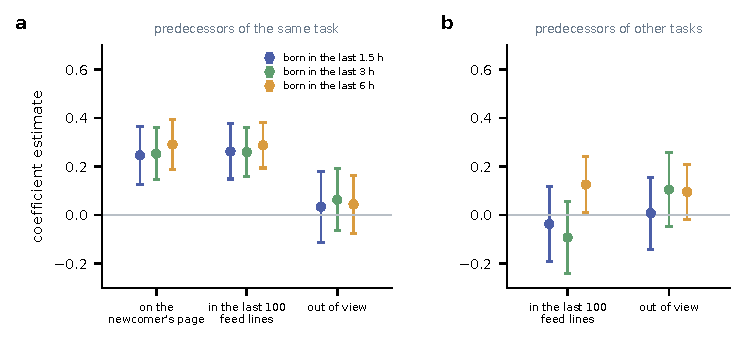
\includegraphics[width=0.85\textwidth]{figs/figS_names_visibility.pdf}
\caption{\textbf{Names respond to the task-mates in view, at three windows.} Coefficients of a linear probability model of whether a newcomer's name carries a feature on the share of the feature among its predecessors, with feature and task by three-hour fixed effects, for predecessors born in the previous 1.5, 3 and 6~h. (a) Predecessors of the newcomer's own task, split into the authors of the page the newcomer wrote on, the handles of the last 100 feed lines, and those out of view. (b) Predecessors of other tasks, in the feed and out of view. Bars are 95\% intervals, clustered by handle.}\label{ed:visibility}
\end{figure}
\begin{figure}[htbp]\centering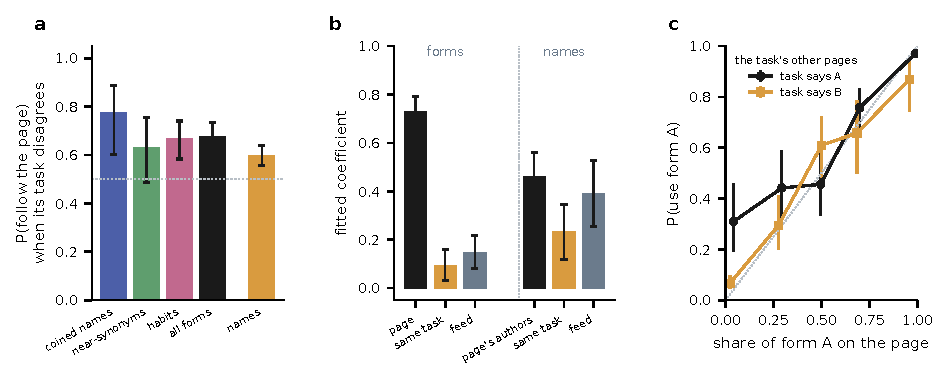
\includegraphics[width=\textwidth]{figs/figS_family.pdf}
\caption{\textbf{The page beats the other pages of its task.} (a) Probability of following the page when the page majority and the majority on the other pages of the same task disagree, for first uses of the three classes and pooled, and for name features when the page's authors and the task-mates of the previous six hours disagree; 95\% Wilson intervals, the dotted line is chance. (b) Coefficients of a joint least squares fit of the outcome on the share on the page, on the other pages of the same task and in the feed, for forms (first uses with at least three instances in each exposure) and for name features; bars are 95\% intervals. (c) The response to the page share, for first uses whose exposure on the task's other pages leans to form A (black) and to form B (amber); the dotted line is proportionality.}\label{ed:family}
\end{figure}
\begin{figure}[htbp]\centering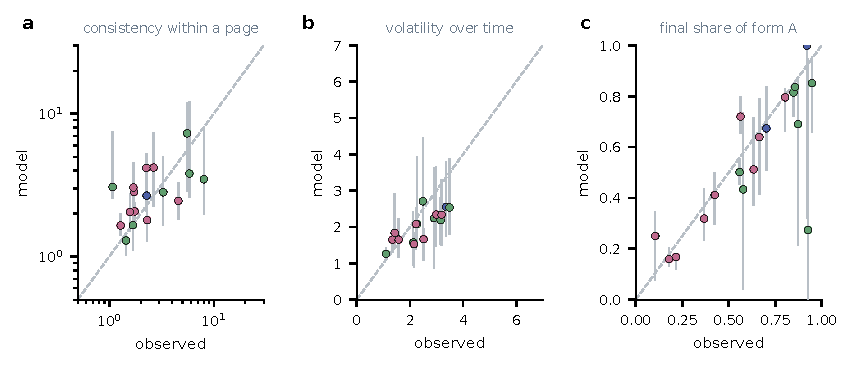
\includegraphics[width=0.9\textwidth]{figs/figS_perconv.pdf}
\caption{\textbf{Each convention against the model run at its own fitted base probabilities.} Median over 50 runs against the observed value, with the 10th to 90th percentile of the runs, for (a) the consistency within a page, (b) the volatility over time, on first uses, and (c) the final share of form A. Colours give the class of the convention. The dashed line is equality.}\label{ed:perconv}
\end{figure}

\end{document}
